%!TEX root = ../main.tex

\chapter{Code generation}
\label{sec:code-generation}

\begin{picture}(0,0)
\put(150,85){\hbox{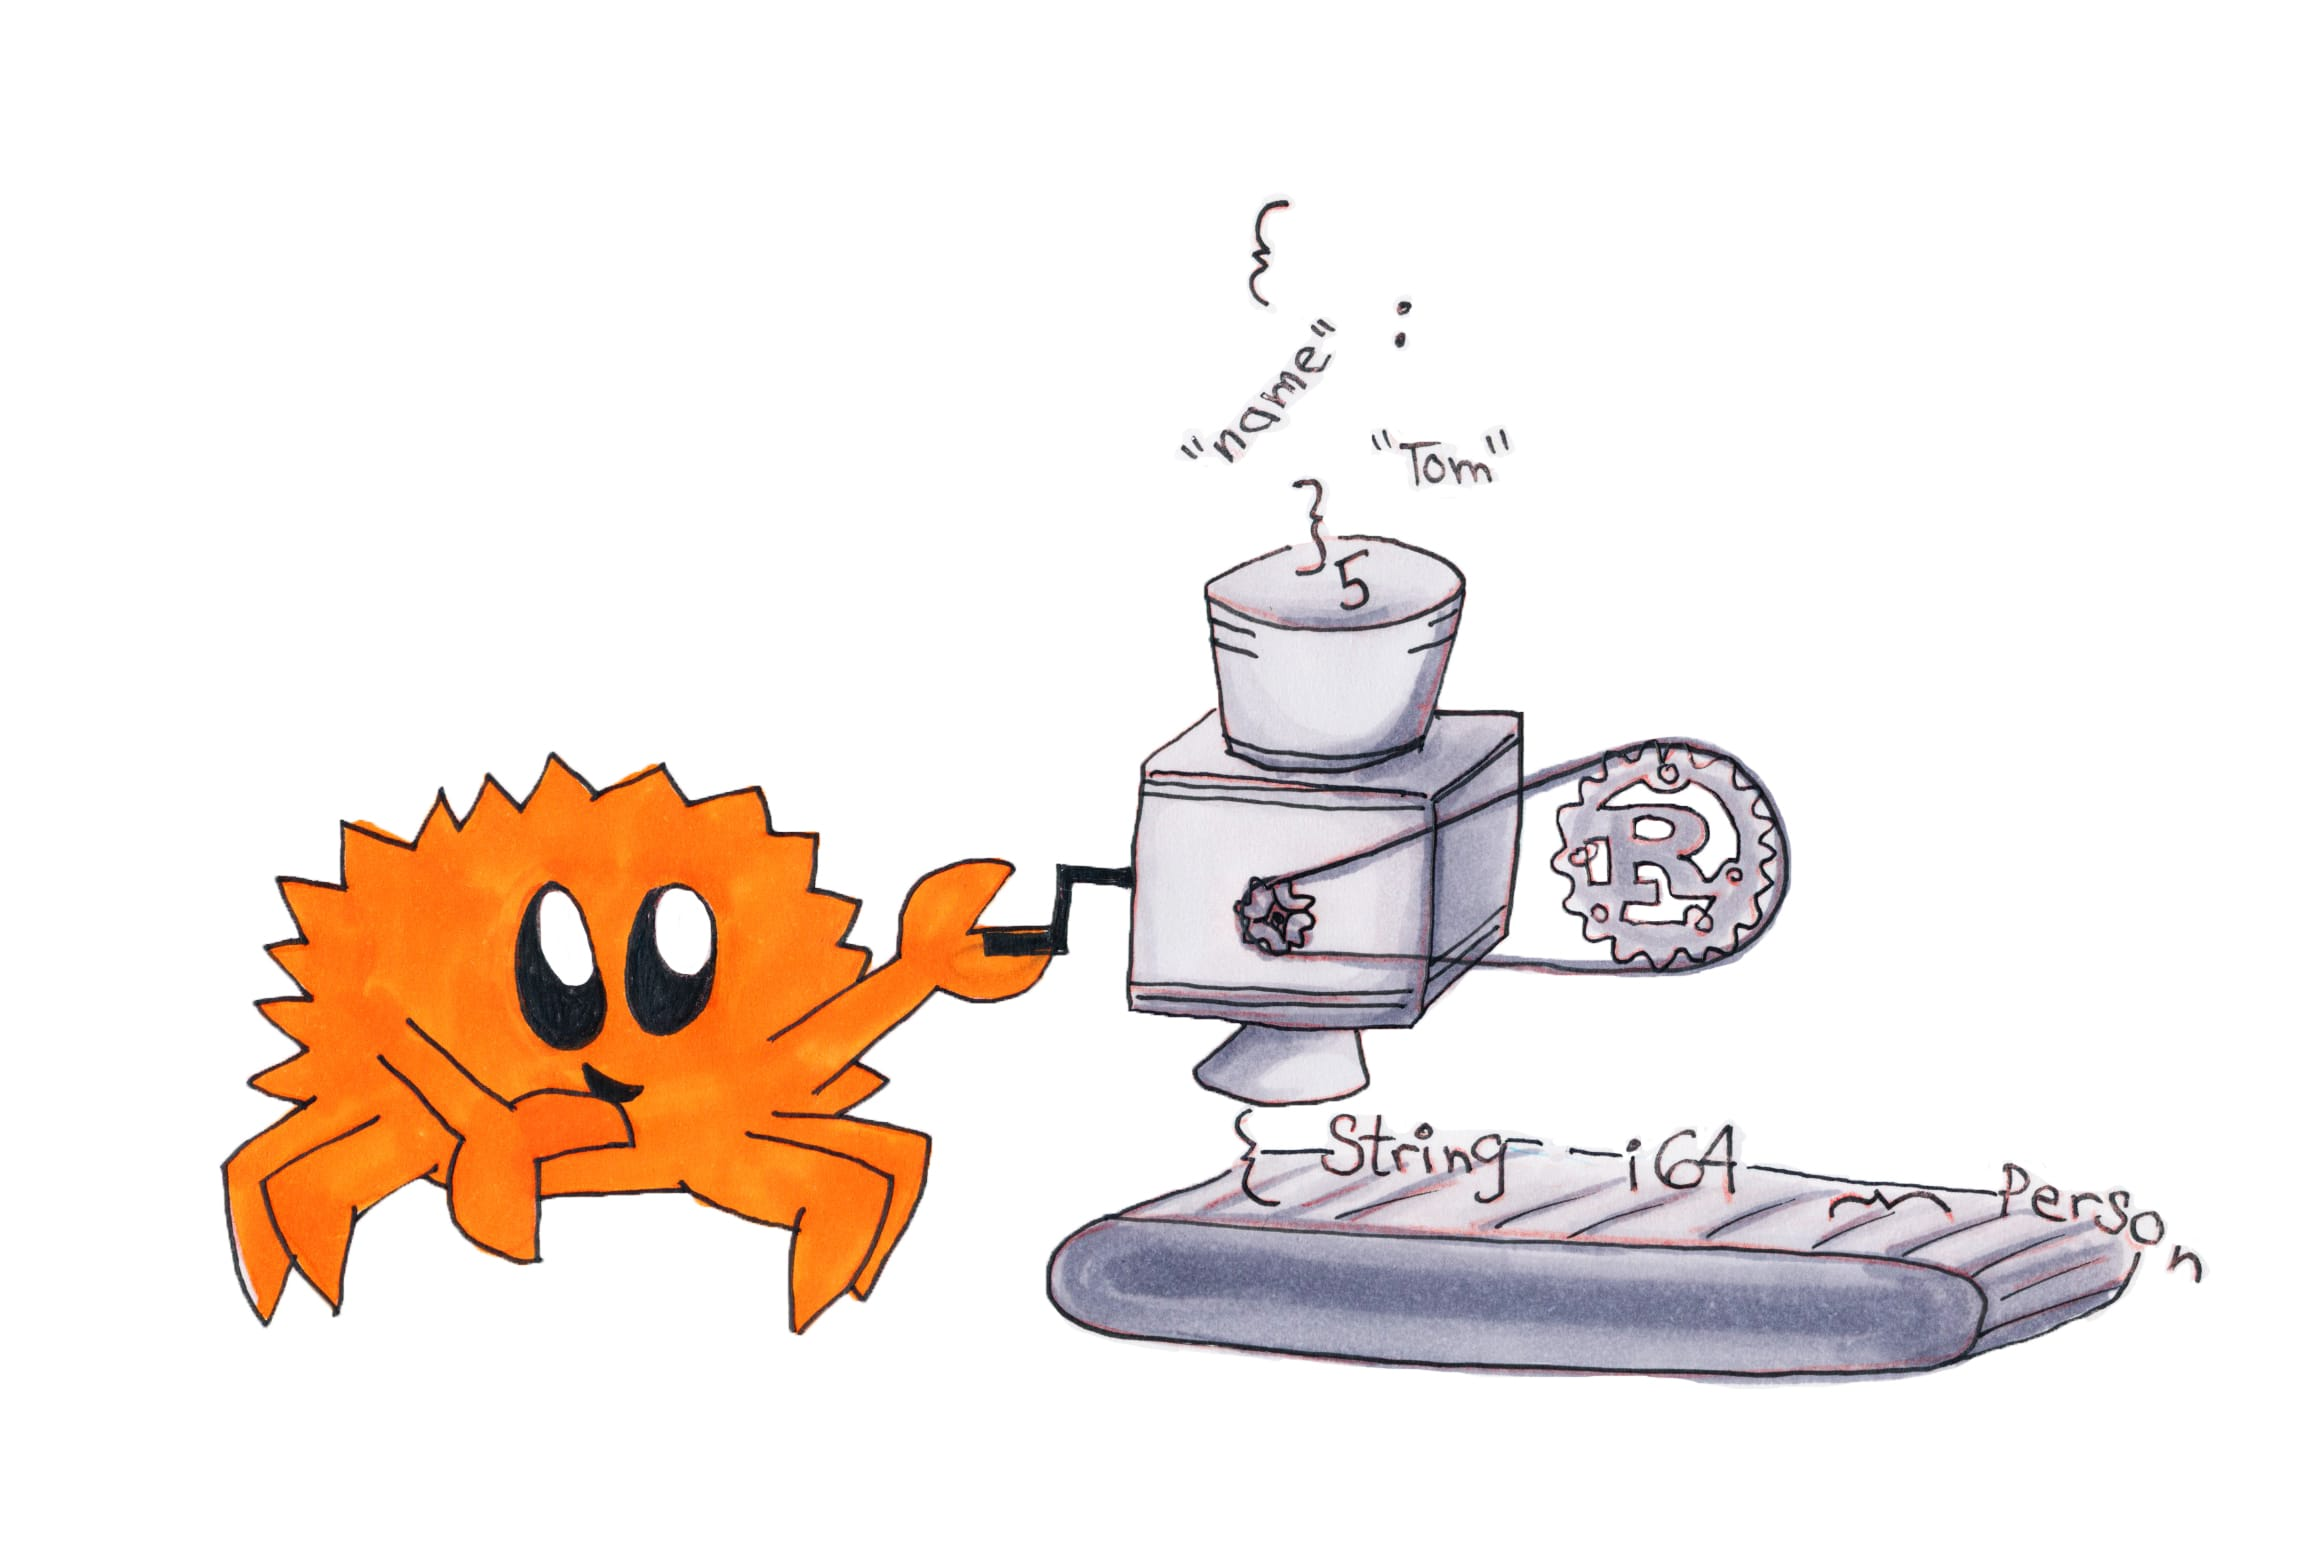
\includegraphics[width=8.5cm, angle=0, trim=40 100 40 40, clip]{ferris/machine}}}
\end{picture}
\vspace{-1cm}

Once a JSON sample has been retrieved and parsed using «serde_json» into the catchall type ‹serde_json::Value›, «json_typegen» is ready to begin inference and code generation. In this chapter we will look at the details of these three stages:

\begin{itemize}
  \item First, a generalized \say{shape} is inferred from the JSON values.
  \item Then this inference is enhanced in intermediary passes.
  \item Finally, Rust code is generated based on the inferred shapes.
\end{itemize}

To begin with I will present a basic version of the inference algorithm and code generation, before looking at how this system can be extended in various ways.

\section{Shape inference}
\label{sec:shape-inference}

The shape inference is based on the algorithms used in \fsharpdata\ as presented in the paper \emph{Types from Data: Making Structured Data First-class Citizens in F\#}\cite{fsharp-types-from-data}. As done in this paper I will use the term shape for the intermediate representation of the inference data, to avoid confusion with actual programming language types.

The goal of the shape inference is to infer generalized shapes from the samples which can then later be used for generating code. These shapes are intended to be general enough to not be tied to inference from JSON -- \fsharpdata\ also does inference for CSV and XML -- and not tied to the generation of any particular type of programming language. Rust code for the basic version of the shape inference can be seen in appendix~\ref{app:inference-code}.

\subsection{Values and shapes}

The inference thus works with two types. The JSON sample, in our case parsed into a ‹serde_json::Value› -- as was shown in listing~\ref{lst:valueenum} -- and the shape type. An abstract version of ‹serde_json::Value›, with value variables \omega, and our shape type, with shape variables \sigma, can be written as follows:

\begin{align*}
\omega ::=  &\ ‹Null› \mid ‹Bool(›b‹)› \mid ‹Number(›n‹)› \mid ‹String(›s‹)› \\
       \mid &\ ‹Array(›[\omega_1, \cdots, \omega_n]‹)› \mid ‹Object(›\{ k_1 : \omega_1, \cdots, k_n : \omega_n \}‹)›\\
\\
\sigma ::=  &\ ‹any› \mid \bot \mid ‹bool› \mid ‹string› \mid ‹int› \mid ‹float› \\
       \mid &\ ‹optional(›\sigma‹)› \mid \vect{\sigma} \mid \recd{ k_1 : \sigma_1, \cdots, k_n : \sigma_n }
\end{align*}

To be clear about how notation is disambiguated: $[a, b, c]$ is an actual sequence of items, while $\vect{a}$ is the \emph{shape} representing a sequence/list.\footnote{In «Types from Data» the notation $\vect{a}$ is used for a different purpose in a section of the paper we will not look at here.} Likewise $\{ k_1 : v_1, \cdots, k_n : v_n \}$ is a map-like collection, while $\recd{ k_1 : \sigma_1, \cdots, k_n : \sigma_n }$ is the \emph{shape} representing a record/object/struct.

For an intuitive understanding of the more abstract shapes it is helpful to think of what kind of knowledge each shape represents. $\bot$ (read as \say{bottom}) represents the complete lack of knowledge about what type should be inferred. $‹optional(›\sigma‹)›$ represents the knowledge that a type may sometimes be ‹null› or a field may not always be there, i.e. that it is nullable or optional. So $‹optional(›\bot‹)›$ tells us that a type is optional, but that we know nothing else of about its type. The ‹any› shape, on the other hand, represents conflicting information. If we end up with the ‹any› shape it means that the information we have received is not representable by any of the other alternatives. E.g. a type that can be both a ‹string› and an ‹int›.

% Differences from algorithm as presented in Types from Data
Unlike in «Types from Data», to preserve information and let any choice be made in the code generation step, lists\footnote{\ldots\ and with extensions, other collections.} are not considered nullable. In other words, the inference can infer the shape $‹optional(›\vect{\sigma}‹)›$, but it is up to the code generation to decide how to handle the shape. In the default code generation, ‹Option<Vec<T>>› will not be generated, but this can be enabled by configuration (‹optional_collections›).

With this change, a separate ‹null› shape, which the original algorithm has, is no longer necessary. Instead, $\bot$ is not considered nullable either, and $‹optional(›\bot‹)›$ serves the purpose of ‹null›.

\subsection{From values to shapes}

\begin{figure}[ht!]
\begin{align*}
\shap(‹Null›)          &= ‹optional(›\bot‹)› \\
\shap(‹Bool(›b‹)›)     &= ‹bool› \\
\shap(‹Number(›n‹)›)   &= \begin{cases}
  ‹int›   & \text{if } n \in \mathbb{Z} \\
  ‹float› & \text{otherwise}
\end{cases}\\
\shap(‹String(›s‹)›)   &= ‹string› \\
\shap(‹Array(›[\omega_1, \cdots, \omega_n]‹)›) &= \vect{ \fold(\csh, \bot, [\shap(\omega_1), \cdots, \shap(\omega_n)]) } \\
\shap(‹Object(›\{ k_1 : \omega_1, \cdots, k_n : \omega_n \}‹)›) &= \recd{ k_1 : \shap(\omega_1), \cdots, k_n : \shap(\omega_n) }
\end{align*}
\caption{$\shap(\omega)$, the function converting JSON values to shapes}
\label{fig:shap}
\end{figure}

The main inference function $\shap(\omega)$, shown in figure~\ref{fig:shap} takes as its input a value and produces a shape. Values containing other values are converted by applying $\shap$ recursively.

$\fold(\textit{function}, \textit{base}, \textit{sequence})$ is the fold operator\cite{fold-tutorial}, common in functional programming (and available on iterators in Rust). In this case, it reduces a sequence of shapes to a single shape by finding a common shape with the $\csh(\sigma_1, \sigma_2)$ function, which we will look at in the next section. The initial shape is $\bot$, which means that an empty ‹Array› will be represented as the shape $\vect{\bot}$.

\subsection{Finding common shapes}

\begin{figure}[ht!]
\begin{align*}
\csh(\sigma, \sigma)     &=  \sigma          & (eq) \\
\csh(\sigma, \bot)       &=  \sigma          & (bottom) \\
\csh(‹int›, ‹float›)     &= ‹float›          & (num) \\
\csh(\sigma_1, ‹optional(›\sigma_2‹)›) &= \opt(\csh(\sigma_1, \sigma_2))  & (opt) \\
\csh(\vect{\sigma_1}, \vect{\sigma_2}) &= \vect{\csh(\sigma_1, \sigma_2)} & (arr) \\
\csh(\sigma_1 = \recd{ \cdots }, \sigma_2 = \recd{ \cdots }) &= \cfs(\sigma_1, \sigma_2) & (obj) \\
\csh(\sigma_1, \sigma_2) &= ‹any›            & (any)
\end{align*}
\caption{$\csh(\sigma_1, \sigma_2)$, the common shape function}
\label{fig:csh}
\end{figure}

Sometimes multiple elements must be represented by the same shape, e.g. a single shape representing all the elements of an array. Figure~\ref{fig:csh} shows the function $\csh(\sigma_1, \sigma_2)$ which for two shapes finds a common shape which can represent them both. Order of arguments does not matter, so for every rule $\csh(a, b)$ the rule $\csh(b, a)$ is the same.

$\csh(\sigma_1, \sigma_2)$ defines a partial order for the set of shapes, where if $\csh(\sigma_1, \sigma_2) \vdash \sigma_3$, $\sigma_1 \sqsubseteq \sigma_3$ and $\sigma_2 \sqsubseteq \sigma_3$. The relation $\sqsubseteq$ can be understood as the \say{can be represented by}-relation. E.g. $ ‹float› \not\sqsubseteq ‹int› $, but $ ‹int› \sqsubseteq ‹float› $ (and also $ ‹int› \sqsubseteq ‹int› $).

\begin{figure}[ht!]
\vspace{2mm}
\centering
\begin{tikzpicture}[>=stealth, thick, shorten >=1pt, auto, scale=1.2]
  \node (bot)     at (8,0) {\bot};
  \node (bot?)    at (9,1) {\bot?};
  \node (int)     at (0,2) {‹int›};
  \node (int?)    at (1,3) {‹int›?};
  \node (float)   at (0,4) {‹float›};
  \node (float?)  at (1,5) {‹float›?};
  \node (bool)    at (2,2) {‹bool›};
  \node (bool?)   at (3,3) {‹bool›?};
  \node (string)  at (4,2) {‹string›};
  \node (string?) at (5,3) {‹string›?};
  \node (arr)     at (6,2) {$\vect{\sigma}$};
  \node (arr?)    at (7,3) {$\vect{\sigma}$?};
  \node (obj)     at (8,2) {$\recd{\cdots}$};
  \node (obj?)    at (9,3) {$\recd{\cdots}$?};
  \node (any)     at (9,6) {‹any›};

  \begin{scope}[on background layer]
    \path[->] (bot)    edge (bot?);
    \path[->] (int)    edge (int?);
    \path[->] (float)  edge (float?);
    \path[->] (bool)   edge (bool?);
    \path[->] (string) edge (string?);
    \path[->] (arr)    edge (arr?);
    \path[->] (obj)    edge (obj?);

    \path[]   (bot)    edge (0,0);
    \path[->] (0,0)    edge (int);
    \path[->] (2,0)    edge (bool);
    \path[->] (4,0)    edge (string);
    \path[->] (6,0)    edge (arr);
    \path[->] (bot)    edge (obj);
    \path[->] (int)    edge (float);

    \path[    dashed] (bot?) edge (1,1);
    \path[->, dashed] (1,1)  edge (int?);
    \path[->, dashed] (3,1)  edge (bool?);
    \path[->, dashed] (5,1)  edge (string?);
    \path[->, dashed] (7,1)  edge (arr?);
    \path[->, dashed] (bot?) edge (obj?);
    \path[->, dashed] (int?) edge (float?);

    \path[]   (float?)  edge (9,5);
    \path[]   (bool?)   edge (3,5);
    \path[]   (string?) edge (5,5);
    \path[]   (arr?)    edge (7,5);
    \path[->] (obj?)    edge (any);
  \end{scope}
\end{tikzpicture}
\vspace{2mm}
\caption{Hasse diagram for the partial order. For compactness $\sigma$? is used for $‹optional(›\sigma‹)›$. Dashed lines are only for visual clarity.}
\label{fig:poset}
\end{figure}

Figure~\ref{fig:poset} shows an incomplete Hasse diagram for the partially ordered set given by $\sqsubseteq$ on the set of shapes. The internal ordering of list and record shapes, $\vect{\sigma}$ and $\recd{\cdots}$, is not shown.

\begin{figure}[ht!]
\begin{align*}
\opt(‹any›)                &= ‹any› \\
\opt(‹optional(›\sigma‹)›) &= ‹optional(›\sigma‹)› \\
\opt(\sigma)               &= ‹optional(›\sigma‹)›
\end{align*}
\caption{$\opt(\sigma)$, the function ensuring optionality/nullability of shapes}
\label{fig:opt}
\end{figure}

When we are working with optional shapes, we want optionality to be a boolean property, i.e. either something is optional, or it is not. For any shape $\sigma$ that already encodes the possibility of values that are missing or ‹null›, $\opt(\sigma)$, as shown in figure~\ref{fig:opt}, is simply a no-op.

\begin{figure}[ht!]
\begin{gather*}
\cfs(\sigma_1 = \recd{ k_1 : v_1, \cdots, k_n : v_n }, \sigma_2 = \recd{ k_1 : v'_1, \cdots, k_n : v'_n }) = \\
\recd[\bigg]{
\forall\ k_n \in \sigma_1 \cup \sigma_2 .\ k_n : \begin{cases}
  \csh(v_n, v'_n) & \text{if } k_n \in \sigma_1 \cap \sigma_2 \\
  \opt(v_n) & \text{if } k_n \notin \sigma_2 \\
  \opt(v'_n) & \text{if } k_n \notin \sigma_1
\end{cases}
}
\end{gather*}
\caption{$\cfs(\sigma_1, \sigma_2)$, the function for finding the common shape of two records}
\label{fig:cfs}
\end{figure}

Figure~\ref{fig:cfs} shows how the common shape of two record shapes is found by finding the common shapes of its fields. For keys that are not present in both records, the shape that is present is optional/nullable. Note that in «Types from Data», records have row variables\cite{row-types} so that all records can be considered to have the same keys. To minimize the number of new concepts needed to understand the basic algorithm I have chosen this slightly less elegant notation in figure~\ref{fig:cfs} instead. Informally, every key present in either of the input record shapes will be present in the output record shape. For every field, if the field is found in both record shapes, the shape of the field in the output is the common shape of the shapes for the corresponding fields in the input. If the field is found in only one of the input shapes, the corresponding field in the output shape must be optional.

\section{Intermediary passes}

In the basic version of the algorithm, there are no intermediary passes. These passes are mainly a result of extensions of the algorithm. The extensions come about for two main reasons: Improving the code to more closely resemble hand-written code, and adding configurability of the inference and code generation.

We will look at these extensions and their consequences for the algorithm in section~\ref{sec:extensions}.

\section{Generating Rust types}

Once a shape tree has been inferred from the sample and intermediate passes have been run to improve the inferred shapes, the shape tree is used to generate Rust code.

The main function takes as its input some path information, used for naming any generated types, and a shape. The function pattern matches on the shape and produces as its output a tuple: The name of the type representing the shape, and potentially some code generated to declare the returned type.

Code is generated via quasiquotation, using a macro ‹quote!› from the «quote»\cite{quote} library.

% TODO: Expand this section

\subsection{Type and field names}

Up to the point of code generation, JSON field names have been preserved as they were in the original JSON. These field names are used to create both field names for the generated types, as well as type names for any nested types. However, as mentioned in section~\ref{sec:json}, the JSON field names can be completely arbitrary strings, while the field names and type names we generated must conform to Rust rules and conventions for identifiers.

The generated names are restricted to consist of \say{words} of alphanumeric ASCII characters, and the complete name must start with a letter. Type names are \say{PascalCased}, i.e. concatenated, with the first letter of each word upper-cased, and field names are \say{snake\_cased}, i.e. all lower case, with words separated by an underscore. For some fields, nothing of the original name remains after restrictions are applied, and we have to resort to fallback names like ‹GeneratedType›.

\begin{listing}[ht!]
\textbf{Sample:}
\begin{minted}{json}
{
  "one two": { " ": 5, "?": 2 }
}
\end{minted}
\vspace{5mm}

\textbf{Generated types:}
\begin{minted}{rust}
struct Root {
    #[serde(rename = "one two")]
    one_two: OneTwo,
}

struct OneTwo {
    #[serde(rename = " ")]
    field: i64,
    #[serde(rename = "?")]
    field2: i64,
}
\end{minted}
\caption{Field and type renaming}
\label{lst:names}
\end{listing}

Additionally the generated types cannot collide with Rust keywords or each other. Collisions with keywords are solved by appending a word describing its use, like ‹field›, so the field ‹"type"› becomes ‹type_field›. Collisions between generated names are solved by adding an incrementing counter to the name.

For field names, if the Rust field name does not match the JSON field name an annotation to relay this information to «Serde» is added to the field. Listing~\ref{lst:names} shows an example with several of these issues at once.

\subsection{Generation of a runnable program}

In addition to just generating the types themselves, the code generation can also generate a complete, runnable Rust program. In addition to the generated types, the runnable program contains the necessary imports and a main function showing how to use «serde_json» to deserialize and serialize into the generated types.

The generation of a full program is mainly for documentation and demonstration purposes in the web interface. Using a button in the web interface the generated code can be directly compiled and run in the online Rust playground.

\subsection{Use of derivable traits}
\label{sec:use-of-derivable-traits}

As outlined in section~\ref{sec:derive-list} a lot of the functionality of «json_typegen» is founded on the fact that many traits can be derived -- i.e. that they can be implemented by just adding their name to a list -- and that this works even for complex generated types.

The fact that this is possible relies on two important preconditions:

\begin{enumerate}
  \item That our generated types are composed of either our base types, or other generated types. I.e. that every leaf in our generated type tree is one of our base types.
  \item That every trait in our derive list is derivable and implemented for each of our base types.
\end{enumerate}

% Proof of "every leaf in our generated type tree is one of our base types" necessary?

% Proof by structural induction here of the claim that this then makes deriving safe for complex types?

Both of these preconditions can be broken by the user if the right configuration option is provided. As explained in section~\ref{sec:derive-list}, the derive list can be overridden. This can obviously break our second precondition, either if a trait is not implemented for one of our base types, or for that matter if the trait is not derivable at all. There are also ways configuration can introduce new, essentially opaque, types into the code generation. These new types essentially become new base types, and as such can easily break our first precondition.

If a user breaks our preconditions in this way and this leads to a compiler error. The messages when a derive fails are clear and should make it quite obvious to the user what the problem is. With this in mind, I think letting the user break these preconditions is an acceptable trade-off for the benefit these configurations provide.

While letting the user break these preconditions is acceptable, care has to be taken to preserve these preconditions when extending the basic system. To make the source of any errors obvious, no derive errors should be possible that does not directly mention a trait or type explicitly specified by the user. E.g. if the system is extended with sets, enabling this extension should not be possible without explicitly choosing a target type if doing so breaks the preconditions.

\subsection{Strictness of deserialization}
\label{sec:design-considerations}

While the types we generate should match the samples they are generated from, and any JSON text that matches their structure, there is always the possibility that the actual JSON we encounter at runtime does not perfectly match what we inferred.

\subsubsection{Mismatched field types}

If a field has entirely the wrong type, e.g. an object where we expect a number, deserialization has to fail with an error, as discovering such type issues as early as possible is a big part of the reason to deserialize to strong types. There are, however, some types we \emph{could} conceivably coerce between. E.g. the string value ‹"3.5"› could be parsed and coerced into a ‹f64› field. While I have some ideas for extensions for specific instances like strings to number, I have no plans for supporting coercing data at runtime in an ad-hoc fashion.

When it comes to how we handle fields that are either missing or that we never saw in inference there are some choices to be made.

\subsubsection{Missing fields}

In the inference we detect potentially missing fields and encode this information into the shapes. By default, the code generation maps $‹optional(›\sigma‹)›$ to ‹Option<T>›, and if any field that was not inferred to be optional is missing, deserialization fails. However, another way to handle missing fields that «Serde» supports is to use the default value provided by an implementation of the ‹Default› trait. I.e. if a string is missing, use the empty string, if an integer is missing use 0, and so on. By enabling this functionality for every field a user could make sure deserialization never fails due to a missing field.

\subsubsection{Additional fields}

By default, if «Serde» tries to deserialize and the data has an additional field that the target type does not have, the additional field is just ignored. This matches well with our intent with type providers, in that we only want to check the assumptions we actually make. However, it is also possible to make such additional fields cause deserialization to fail.

\section{Extensions}
\label{sec:extensions}

As have been mentioned earlier, there are several ways to extend this basic setup to better align with what handwritten code would look like. We will now look at a few such extensions. For the sake of simplicity, we will mostly not go into the details of how these extensions interact or the complete extended algorithms, focusing instead on each extension by itself.

\subsection{Tagged any types}
\label{sec:tagged-any}

In addition to the basic inference algorithm described in section~\ref{sec:shape-inference}, «Types From Data»\cite{fsharp-types-from-data} also describes an extension it calls \say{labelled top shapes} for providing a better fallback than the general ‹any› shape.

In the basic algorithm, if the least upper bound given by $\csh(\sigma_1, \sigma_2)$ is ‹any›, we throw away the information we have about why we had to use ‹any›, i.e. $\sigma_1$ and $\sigma_2$. The basic concept of this extension is to instead incorporate this information into a top type $‹anyof(›\sigma_1, {\cdots}, \sigma_n‹)›$. This can then be used in the code generation to e.g. create enumerated types with custom types inside.

% TODO: Show how a type generated from an anyof shape could look

% TODO: HTML or XML example

This extension is absolutely vital for making the algorithm work well with XML and HTML. In these formats heterogeneous collections with easily disambiguated types are abundant. For «json_typegen», the extension is still useful, but less important than some other extensions.

\subsection{JSON pointer hints and configuration}
\label{sec:ext-json-pointers}

As outlined in section~\ref{sec:json-pointers} we can use JSON pointers to specify configuration options and hints to the inference that are specific to just a part of the JSON sample.

Actually applying these options and hints require some modifications to the basic version of the algorithm.

Some have to be applied during inference, some are best applied as intermediate transformations between inference and code generation, and some have to be applied during the code generation.



% some in inference, some as intermediate steps, some for

% consequences of plain pointers (and array indexes), full wildcards and partial wildcards

% same_as, ids to see which types are the same

\subsection{More number types}
\label{sec:unsigned}

% By default, our code generation only uses ‹i64› for integers and ‹f64› for floating point numbers...

Rust supports unsigned integers. By default we do not infer unsigned integers. The primary benefit of unsigned numbers is to disallow negative values, but while it is common to write floating point numbers with the decimal point even when the value is an integer, there is no such hint for numbers which may be negative. As such the risk/reward is just not good enough to justify it as a default.

While unsigned numbers are not enabled by default, like $‹optional(›\vect{\sigma}‹)›$, an ‹unsigned› shape can just be inferred and not used unless manually enabled.

\subsection{Maps}
\label{sec:ext-maps}

One common issue with JSON is that its simplicity means that some common data structures are missing. This drives people to use the same data structures with different intentions as different ad-hoc data structures. Perhaps the most common such pattern is the use of JSON objects as maps.

% Should the concept of a map be explained?

While JSON has no concept of a map, maps with strings as keys can be encoded in JSON as objects, and there is no loss of fidelity inherent in this encoding. The only issue for us is that there is no good way to infer the difference between an object used to encode a structure that will persist across e.g. API calls, and an object used to encode a mapping from arbitrary keys to values.

% "Impossible" to infer, but can be hinted.
While the intention that an object is used as a map can not be directly inferred from just a sample, with inference hints from the user, code using maps can still be inferred and generated.

\begin{figure}[ht!]
\begin{gather*}
\shap(‹Object(›\{ k_1 : \omega_1, \cdots, k_n : \omega_n \}‹)›, [\cdots, ‹"" use_type map›, \cdots]) = \\
‹map(›\fold(\csh, \bot, [\shap(\omega_1), \cdots, \shap(\omega_n)])‹)› \\
\shap(\omega, [\cdots, ‹"" use_type map›, \cdots]) = ‹error!›
\end{gather*}
\caption{Extending the hinted $\shap$ to support maps}
\label{fig:shap-map}
\end{figure}

\begin{figure}[ht!]
\begin{align*}
\csh(‹map(›\sigma_1‹)›, ‹map(›\sigma_2‹)›) &= ‹map(›\csh(\sigma_1, \sigma_2)‹)›     & (map)
\end{align*}
\caption{Extending $\csh$ to support maps}
\label{fig:csh-map}
\end{figure}

To be able to infer maps we would first need to add $‹map(›\sigma‹)›$ as an alternative to our set of possible shapes. In the notation I have not included the key type, as JSON only supports string keys for object fields, and as such to assume strings as map keys in the generated code should suffice. Figure~\ref{fig:shap-map} shows how the function $\shap$ already extended with hints could be extended to infer maps. The shown rules should take priority over the existing rule matching on ‹Object›.

% Values in a map are essentially already nullable.
$\csh$ can be extended by adding a simple rule shown in figure~\ref{fig:csh-map} before the existing rule $(any)$. One may argue that map values are already nullable, since ‹map.get()› or any equivalent will return some nullable type, and that we should thus take care to not infer a shape for the map values which could be lowered to a non-nullable shape (or rather, to lower such types when we infer them).

However, the only nullable shape we currently have that can be lowered to something else is $‹optional(›a‹)›$, which can be lowered to its wrapped shape $a$. The only way for the algorithm to infer map values that are $‹optional(›a‹)›$ is if the map sample contains explicit ‹Null› values. For a map to contain such values would be quite rare, and if it were to happen, those null values are likely to carry meaning. With these things in mind, I consider the best option to be to \emph{not} lower the map value shapes.

In most programming languages there is also the consideration of which map type to use. The Rust standard library provides two map types, ‹HashMap› and ‹BTreeMap›. In addition to these alternatives there are various map types in published in crates in the Rust ecosystem. As an example, «json_typegen» itself uses a ‹LinkedHashMap› internally. From the perspective of a user, giving a hint $‹use_type›\ t$ should work with any of the types mentioned above for $t$, as well as just ‹map›, letting «json_typegen» choose the map type.

For the default map type, whatever we choose ends up as essentially a new base type. Both ‹HashMap› and ‹BTreeMap› are good candidates, but as the default I have chosen ‹HashMap›, as it is the recommendation for general maps.\cite[std::collections]{rust-std-docs}. As mentioned, we assume strings as keys, so the full new base type is ‹HashMap<String, T›. With ‹String› fixed as the key type, ‹HashMap› implements all the traits in our derive list and can thus be safely added to our set of base types.

% Whatever type json_typegen chooses ends up as part of our base types.
% HashMap<String, T> implements all of Default, Debug, Clone, PartialEq, Serialize, Deserialize

% Show how we split apart use_type HashMap into use_type map for inference algo and use_type HashMap for typegen.

\subsection{Tuple types}
\label{sec:ext-tuples}

Another common pattern of data structure adaption in real world JSON is the use of arrays as tuples. E.g. serializing the tuple ‹("a", 1)› as the JSON text ‹["a", 1]›. Unfortunately, this does not interact very well with the basic algorithm. The JSON text ‹["a", 1]› would be inferred as the shape $\vect{‹any›}$. Rust does, however, have tuples, and could represent the type as ‹(String, i64)›, so if it is possible to do so without breaking the original algorithm it makes sense to try to infer tuples.

\begin{figure}[ht!]
\begin{gather*}
\shap(‹Array(›[\omega_1, \cdots, \omega_n]‹)›) = \\ \begin{cases}
  \tupl{ \shap(\omega_1), \cdots, \shap(\omega_n), 1 }   &  \text{if } 1 < n \leq tmax \\
  \vect{ \fold(\csh, \bot, [\shap(\omega_1), \cdots, \shap(\omega_n)]) } & \text{otherwise}
\end{cases}
\end{gather*}
\caption{$\shap(\omega)$, rule modification for tuples}
\label{fig:shap-tuple}
\end{figure}

To be able to infer tuples we add the tuple shape $\tupl{ \sigma_1, \cdots, \sigma_n, \kappa }$ to our set of shapes, where $ \sigma_1, \cdots, \sigma_n $ are field shapes and $\kappa$ is the count of samples this shape is based on. Figure~\ref{fig:shap-tuple} shows how $\shap(\omega)$ can be modified to infer tuples. The shown rule replaces the original rule for ‹Array›.

A tuple automatically implements all the traits in our default derive list if all the types inside it does\cite[primitive std::tuple]{rust-std-docs}, and so can be safely added to our set of base types. This derive-like functionality only works for tuples with at most 12 fields, so the max inferred tuple arity -- $tmax$ -- should never be set higher than this. In my own opinion, anything beyond 2-tuples and 3-tuples should not be automatically inferred.

\begin{figure}[ht!]
\begin{gather*}
\csh(\tupl{ \sigma_1, \cdots, \sigma_n, \kappa_1 }, \tupl{ \sigma'_1, \cdots, \sigma'_m, \kappa_2 }) = \\
\begin{cases}
  \tupl{ \csh(\sigma_1, \sigma'_1), \cdots, \csh(\sigma_n, \sigma'_m), \kappa_1 + \kappa_2 }   &  \text{if } n = m \\
  \vect{ \csh(\fold(\csh, \bot, [\sigma_1, \cdots, \sigma_n]), \fold(\csh, \bot, [\sigma_1, \cdots, \sigma_n])) } & \text{otherwise}
\end{cases} \\
\csh(\tupl{ \sigma_1, \cdots, \sigma_n, \kappa }, \vect{\sigma_m}) = \\
\vect{\csh(\fold(\csh, \bot, [\sigma_1, \cdots, \sigma_n]), \sigma_m)}
\end{gather*}
\caption{$\csh(\sigma_1, \sigma_2)$, rule additions for tuples}
\label{fig:csh-tuple}
\end{figure}

Figure~\ref{fig:csh-tuple} shows how $\csh(\sigma_1, \sigma_2)$ can be extended to accommodate for tuples. The two rules are pure additions, and none of the original rules are affected.

% [1, 2] => [int]
% [[1, 2], [3, 4]] => [(int, int)]
% [1, "foo"] => (int, string)

\begin{figure}[ht!]
\begin{gather*}
\text{tolist}(\tupl{ \sigma_1, \cdots, \sigma_n, \kappa }) = \vect{\fold(\csh, \bot, [\sigma_1, \cdots, \sigma_n])} \\ \\
\text{test}(\sigma_t = \tupl{ \sigma_1, \cdots, \sigma_n, \kappa })  = \\
\kappa \geq tsamplemin \lor ((\exists \sigma \in [\sigma_1, \cdots, \sigma_n] . \sigma \neq ‹any›) \land \text{tolist}(\sigma_t) = \vect{‹any›})
\end{gather*}
\caption{Removal of tuple shapes}
\label{fig:remove-tuple}
\end{figure}

When we add tuples to the inference, while some tuples can be inferred automatically, our code generation should not be \emph{too} eager to use tuples. We do not want every short list in our samples to be interpreted as a tuple. Figure~\ref{fig:remove-tuple} shows how tuple shapes can be converted to lists, and the test for whether a tuple shape should be used or converted to a list shape. Intuitively, a tuple shape should only be used if we have either seen enough instances to believe it is not just a short list, or if the use of a tuple type will prevent us from combining shapes into the fallback shape ‹any›. Note that the clause $(\exists \sigma \in [\sigma_1, \cdots, \sigma_n] . \sigma \neq ‹any›)$ will be redundant if we consider 2 to be enough samples to use a tuple.

If automatic inference of tuples is disabled, tuple shapes can still be created, and every tuple shape encountered in code generation can be converted to a list unless locally enabled by pointer configuration.

\subsection{Combining identical subtypes}

Finding identical subtypes is the task of finding identical subtrees in our shape tree. A naive approach needs $\binom{n}{2} = \frac{n(n-1)}{2} \in O(n^2)$ comparisons, so care must be taken on implementation. Our shape tree can be considered to be a rooted unordered labelled tree. Finding identical types would still be somewhat useful even if we consider the tree ordered, so this could be done to make initial implementation easier.

\placeholder{Inferring types from multiple samples/sample-sets but ensuring that they can still work together. Show how this can already be done to a certain extent using \url{https://github.com/lloydmeta/frunk}}

\subsection{Detection of entirely separate types}

When inferring shapes and generating code based on JSON one has to work with incomplete data. As such it is unavoidable that some choices have to be made. Unfortunately several of these choices do not present any alternative that is clearly better in all cases.

\begin{listing}[ht!]
\begin{minted}{json}
[
  {
    "a": 1
  },
  {
    "b": 1
  }
]
\end{minted}
\caption{JSON Dilemma \#1}
\label{lst:json-dilemma-1}
\end{listing}

\begin{listing}[ht!]
\begin{minted}{rust}
struct S {
    a: Option<i32>,
    b: Option<i32>,
}

enum E {
    A { a: i32 },
    B { b: i32 },
}
\end{minted}
\caption{JSON Dilemma \#1 - Two solutions}
\label{lst:json-dilemma-1-rs}
\end{listing}
